\documentclass[14pt,a4paper]{extreport}

\usepackage[utf8]{inputenc}
\usepackage[romanian]{babel}

% \renewcommand\familydefault{\sfdefault} % computer modern sans serif
\usepackage{fontspec}
\setmainfont{Times New Roman}


\linespread{1}

\usepackage{geometry}
 \geometry{
 left=20mm,
 right=10mm,
 top=20mm,
 bottom=20mm,
 % showframe
}

\usepackage{xcolor}
\definecolor{mygreen}{rgb}{0,0.6,0}
\definecolor{mygray}{rgb}{0.5,0.5,0.5}
\definecolor{mymauve}{rgb}{0.58,0,0.82}
\definecolor{darkgray}{rgb}{.4,.4,.4}
\definecolor{navy}{HTML}{000080}
\definecolor{purple}{rgb}{0.65, 0.12, 0.82}
\definecolor{codepurple}{rgb}{0.58,0,0.82}
\definecolor{backcolour}{rgb}{0.95,0.95,0.92}

% Please add the following required packages to your document preamble:
\usepackage{multirow}
\usepackage{array}

\usepackage{caption}
% \usepackage[singlelinecheck=false]{caption}

% \captionsetup[table]{name=Tabelul}

\usepackage{graphicx}
\graphicspath{ {../png} }

\usepackage{amsmath} % for the equation* environment

\usepackage{xcolor}   % for \textcolor
\usepackage{listings}
\definecolor{codegreen}{rgb}{0,0.6,0}
\definecolor{codegray}{rgb}{0.5,0.5,0.5}
\definecolor{codepurple}{rgb}{0.58,0,0.82}
\definecolor{backcolour}{rgb}{0.95,0.95,0.95}

\lstset{
    backgroundcolor=\color{backcolour},   
    commentstyle=\color{codegreen},
    keywordstyle=\color{magenta},
    numberstyle=\color{navy},
    stringstyle=\color{codepurple},
    breakatwhitespace=false,         
    breaklines=true,                 
    captionpos=b,                    
    keepspaces=true,                 
    numbers=left,                    
    numbersep=5pt,                  
    showspaces=false,                
    showstringspaces=false,
    showtabs=false,                  
    tabsize=2,
  columns=fullflexible,
  frame=single,
  breaklines=true,
  postbreak=\mbox{\textcolor{red}{$\hookrightarrow$}\space},
}
\usepackage{csvsimple}
\usepackage{float}

\begin{document}

\begin{titlepage}
\begin{center}
	{\large{ Universitatea Tehnica a Moldovei \\}}
	{\large{ Facultatea Calculatoare, Informatică și Microelectronică \\}}
	{\large{ Departamentul Ingineria Software și Automatică \\}}
	\vspace{4cm}
	{\LARGE {\bf{ Raport }}}\\
	\vspace{1cm}
	{\large { Lucrarea de Laborator Nr.4 \\}}
	{\large { Analiza și Proiectarea Algoritmilor \\}}
	{\large { Tema: Metoda programării dinamice   \\}}
\end{center}

\vspace{5cm}

\noindent{\large A efectuat:\hfill St. gr. TI-206} \\
\noindent{\large\null\hfill Pleșu Cătălin} \\
\noindent{\null} \\
\noindent{\large A verificat:\hfill Lect. Univ.} \\
\noindent{\large\null\hfill Bîtca Ernest} \\

\vspace{5cm}

\centering{\large{ Chișinău 2021 }}
\end{titlepage}


\clearpage
\subsection*{Scopul:\\}
\begin{enumerate}
	\item Studierea metodei programării dinamice.
	\item Analiza şi implementarea algoritmilor de programare dinamică. 
	\item Compararea tehnicii greedy cu metoda de programare
\end{enumerate}

\subsection*{Sarcina:}
\begin{enumerate}
	\item De studiat metoda programării dinamice de proiectare a algoritmilor. 
	\item De implementat într-un limbaj de programare algoritmii prezentaţi mai sus. 
	\item De făcut analiza empirică a acestor algoritmi pentru un graf rar şi dens.
\end{enumerate}
 
\clearpage
\subsection*{ Întrebări de control: \\}
\begin{enumerate}
	\item Descrieţi metoda programare dinamică. 
	\item De ce această metodă se numeşte programare dinamică? 
	\item Care este diferenţa între metoda divide et impera şi metoda programării dinamice? 
	\item Care este clasificarea problemelor de programare dinamică? 
	\item Ce se întâmplă în cazul când costurile arcelor grafurilor prelucrate cu algoritmii Dijkstra şi Floyd sunt negative? 
\end{enumerate}

\begin{enumerate}
	\item Programarea dinamică este în principal o optimizare față de recursiunea simplă. Ori de câte ori vedem o soluție recursivă care are apeluri repetate pentru aceleași intrări, putem optimiza folosind programarea dinamică. 
	\item Cuvântul dinamic a fost ales de Bellman pentru a captura aspectul variabil al problemelor și pentru că a sunat impresionant.
	\item Diferența între metoda divede et impera și metoda programării dinamice este că ultima nu folosește recursii pentru a rezolva problemele.
	\item Există mai multe clasificări ale problemelor de programare dinamică: 
	 \begin{enumerate}
		 \item După  natura deciziilor pot fi deterministe sau nedeterministe.  La cele nedeterministe, în scrierea relaţiilor de recurenţă intervine şi o probabilitate (probabilitatea ca produsul să fie vândut, ca individul x să ajungă într-un punct dat, ca moneda să cadă pe partea cu stema, ca o maşină să se strice după ce a produs un număr de piese.) 
		 \item După valoarea deciziilor pot fi de optimizare (determinarea drumurilor de cost minim între două noduri ale unui graf), de neoptimizare (determinarea numerelor Fibonacci).   
		 \item După numărul de dimensiuni (sau numărul de parametri ai funcţiilor de recurenţă) pot fi unidimensionale (precum numerele lui, sau multidimensionale. 
		 \item După numărul deciziilor care se pot lua la un pas pot fi unidecizionale (ca numerele lui Fibonacci), sau multidecizionale (ca drumul de lungime minimă între două noduri ale unui graf).  Problemele unidecizionale sunt de obicei de neoptimizare. 
		 \item După direcţia deciziilor putem avea programare dinamică înainte în care starea i se calculează în funcţie de stările  i + 1, i + 2, …, sau programare dinamică înapoi în care starea i  se calculează în funcţie de stările i – 1, i – 2, ….   
	 \end{enumerate}
 \item În cazul în care grafurile ar avea costuri negative algoritmul Dijkstar nu ar funcționa corect pe când algoritmul floyd ar funcționa cum ne așteptăm.
\end{enumerate}

\clearpage
\subsection*{Testarea empirică a algoritmilor}
%cazul 1
\subsection*{}{
\begin{table}[h]
\captionsetup{singlelinecheck = false, justification=raggedright}
	\caption{Timpul de rulare pentru graf rar}
\label{tab:rare} 
\begin{center}
	\csvautotabular{../rare.csv}
\end{center}
\end{table}

\paragraph{}
\begin{figure}[H]
\begin{center}
	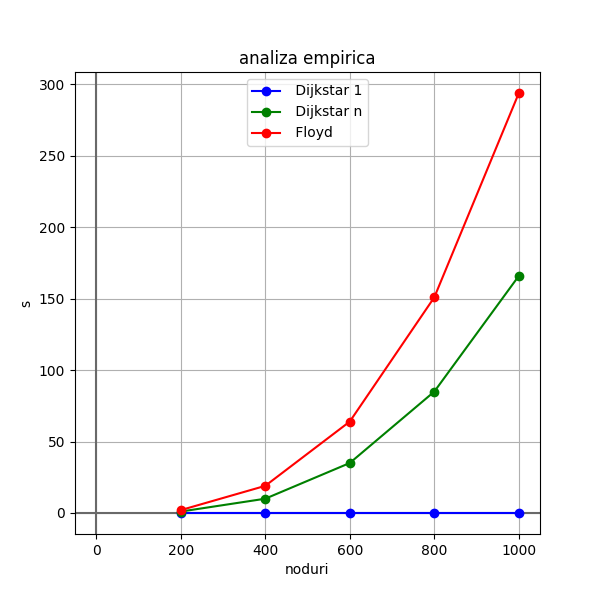
\includegraphics[width=14cm]{rare}
	\caption{Timpul de rulare din tabela ~\ref{tab:rare}} 
	\label{fig:rare} 
\end{center}
\end{figure}
\paragraph{}
După cum se observă în Figura ~\ref{fig:dense} algoritmul Floyd este mai ineficient decât algoritmul Dijkstra, totodată algoritmul Dijkstra mai are un avantaj, el poate fi rulat doar pentru un vârf astfel timpul lui de execuție fiind neglijabil pentru cazurile noastre.
}
%cazul 2
\subsection*{}{
\begin{table}[h]
\captionsetup{singlelinecheck = false, justification=raggedright}
	\caption{Timpul de rulare pentru graf dens}
	\label{tab:dense} 
\begin{center}
	\csvautotabular{../dense.csv}
\end{center}
\end{table}

\paragraph{}
\begin{figure}[H]
\begin{center}
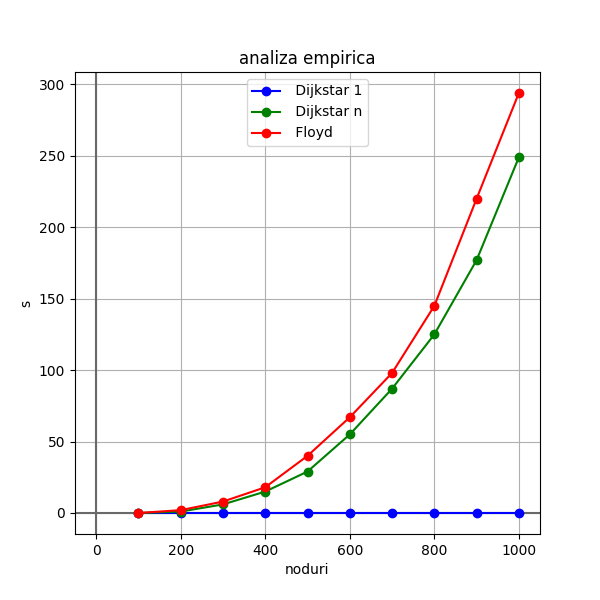
\includegraphics[width=14cm]{dense}
	\caption{Timpul de rulare din tabela ~\ref{tab:dense}} 
	\label{fig:dense} 
\end{center}
\end{figure}
\paragraph{}
După cum se observă în Figura ~\ref{fig:dense} analizând această figură putem observa că în mărimea problemei algoritmului Dijkstra sunt sunt incluse si numărul de muchii, pe când algoritmul folyd depinde doar de vârfuri, și execuția lui nu diferă de graful rar.
}

\clearpage
\subsection*{Testarea programului}
\paragraph{}
Pentru testarea corectitudinii programului voi introduce în program un graf de 6 vârfuri care a fost rezolvat precent cu metoda dijkstra si voi compara rezultatele.

\begin{figure}[H]
\begin{center}
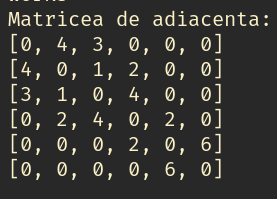
\includegraphics[width=10cm]{adiacence}
	\caption{Matricea de adiacență} 
\end{center}
\end{figure}

\begin{figure}[H]
\begin{center}
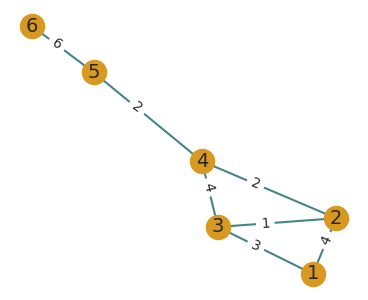
\includegraphics[width=14cm]{graf}
	\caption{Graful} 
\end{center}
\end{figure}

\begin{figure}[H]
\begin{center}
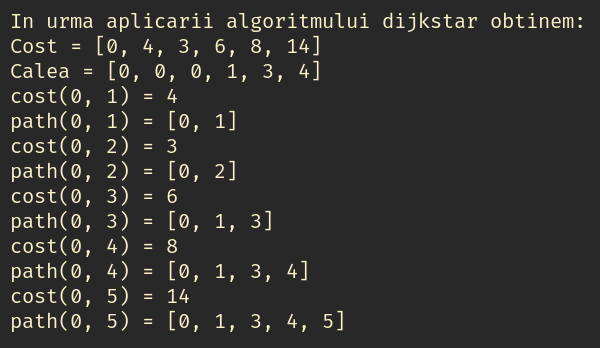
\includegraphics[width=14cm]{dijkstra}
	\caption{Algoritmul Dijkstra} 
\end{center}
\end{figure}

\begin{figure}[H]
\begin{center}
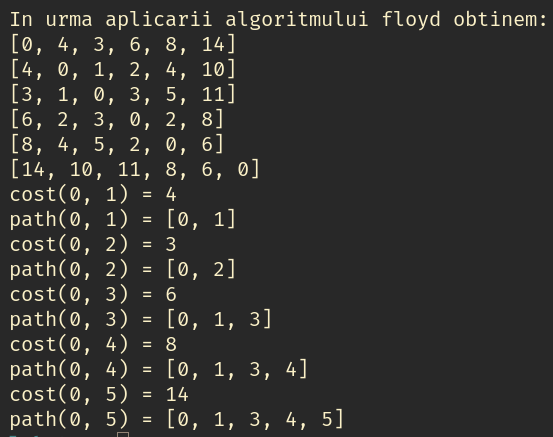
\includegraphics[width=14cm]{floyd}
	\caption{Algoritmul Floyd} 
\end{center}
\end{figure}

\clearpage
\subsection*{Concluzii:}
\paragraph{}
În cadrul acestei lucrări de laborator am implementat un algoritm greedy și un algoritm dinamic, dijkstar și floyd. Ambii algoritmi au puncte tari și slabe. Avantajul algoritmului dijkstra este că poate fi pornit doar pentru vârfurile de care avem nevoie avest lucru scurtând semnificativ timpul de execuție. Avantajul algoritmului floyd e ca poate opera și pe grafuri cu costuri negative.
\paragraph{}
Comparând graficele obținute am ajuns la concluzia că algoritmul dijkstra este mai eficient indiferent grafurile daca dorim sa aflam o cale sau toate căile din graf. Sau o altă concluzie posibilă este că la în codul pentru algoritmul floyd se poate de făcut niște optimizări ca să fie mai eficient fiind că diferența dintre timpul de executare nu este chiar atât de mare.
\paragraph{}
Comparând rezultatele obținute pe cale empirică constatăm că pentru implementarea respectivă algoritmul dijkstra va fi mai eficient decât algoritmul floyd pentru toate cazurile.

\vfill
\begin{flushright}
\LaTeX
\end{flushright}


\appendix
\clearpage
\section*{Anexa main.rs}
\lstinputlisting[frame=none]{../src/main.rs}

\clearpage
\section*{Anexa graph.rs}
\lstinputlisting[frame=none]{../src/graph.rs}

\clearpage
\section*{Anexa dijkstra.rs}
\lstinputlisting[frame=none]{../src/dijkstar.rs}

\clearpage
\section*{Anexa floyd.rs}
\lstinputlisting[frame=none]{../src/floyd.rs}

\clearpage
\section*{Anexa main.py}
\lstinputlisting[language=python, frame=none]{../src/main.py}

\end{document}
